% Notas content

\begin{enumerate}
  \item Como é possı́vel determinar a massa efetiva dos semicondutores com o experimento de ressonância ciclotron? Discuta partindo da equação do movimento de Drude o que é a ressonância ciclotron, e a geometria/consequência experimental.\\

    Nós temos que a força de Loretenz é dada por:

    \begin{equation}
         \mathbf{F} = q(\mathbf{E} + v \times \mathbf{B}) 
    \end{equation}

    Considerando que o campo elétrico, $E$ seja igual a $0$, e usando a definição de força chegamos na expressão (estou negligenciando o termo de amortecimento que aparece na equação de drude, pois ele não irá alterar a frequência final, apenas o pico):

    \begin{equation}
        m^*\dv{v}{t} = q(v \times \mathbf{B}) 
    \end{equation}

    Supondo que temos um campo magnético uniforme na direção $\hat{z}$, ou seja: $\mathbf{B} = B\hat{z}$, podemos dizer então que $v \times B$ é dado por:

    $$(v_x, v_y, 0) \times (0, 0, B) = (v_yB, -v_xB, 0)$$
    Indicando que temos uma rotação no plano xy. Podemos separar as equações diferenciais de acordo com suas componentes, ficamos então com:
  \begin{center}
    $\begin{cases}
      m^*\dv{v_x}{dt} = q(v_yB)\\\\
      m^*\dv{v_y}{dt} = -q(v_xB)
    \end{cases}$
  \end{center}
  
  Podemos derivar a primeira equação diferencial mais uma vez, obtendo então:

  $$m^*\dv[2]{v_x}{t} = qB\dv{v_y}{t}$$
  Porém, sabemos que $\dv{v_y}{t} = -\frac{qB}{m^*}v_x$. Substituindo obtemos no final que:

  \begin{equation}
     \dv[2]{v_x}{t} = -\left(\frac{qB}{m^*}\right)^2v_x 
  \end{equation}

  A forma dessa equação diferencial é a mesma do oscilador harmônico que já resolvemos em aula, sendo assim, podemos definir uma frequência (que parece ser uma convenção nos livros) \textit{ciclotron}:

  \begin{equation}
      \omega^2 = \left(\frac{qB}{m^*}\right)^2 \Implies \omega = \frac{|q|B}{m^*} 
  \end{equation}
  
  No experimento de ressonância ciclotron, a intenção é aplicar um campo eletromagnético com uma frequência $\omega$ até que ela chegue na frequência ciclotron, pois ao terem a mesma frequência, elas entram em ressonância e absorção de energia do elétron é máxima. Nós não sabemos a frequência ciclotron, nem a massa efetiva, porém sabemos que se variarmos a frequência do campo eletromagnético que estamos emitindo, em um dado momento teremos um pico no gráfico $E \times \omega$, e é justamente esse pico que corresponde à frequência ciclotron. Dessa forma, sabendo a frequência, a carga do elétron e o campo magnético, podemos calcular a massa efetiva dos semicondutores.

\item Como é possı́vel determinar a concentração de portadores dos semicondutores usando medidas Hall? Discuta partindo da equação do movimento de Drude a consequência experimental da geometria Hall.


\begin{figure}[htbp]
  \centering
  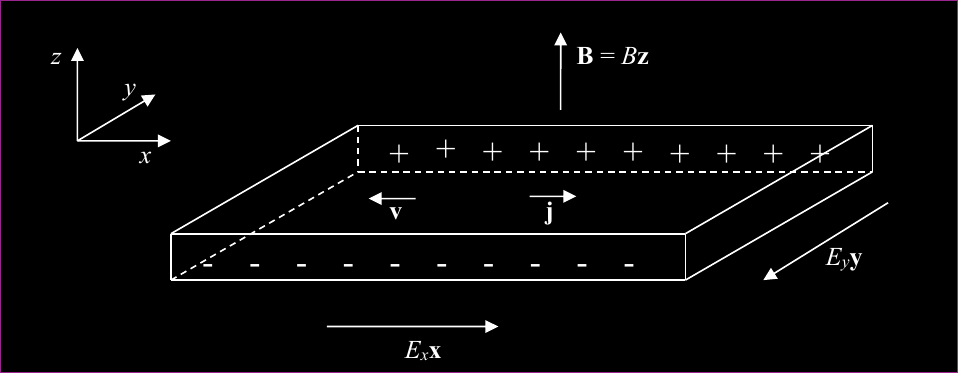
\includegraphics[width=\linewidth]{images/Hall experiment.png}
\end{figure}
  
A geometria do experimento Hall parte do pressuposto que temos dois campos sendo aplicados em nossa amostra, um campo elétrico sendo aplicado na direção +x, $E_x\hat{x}$ e um campo magnético sendo aplicado perpendiculamente, direção z, $\mathbf{B} = Bz$. O campo elétrico $E_x\hat{x}$ faz com que tenhamos uma corrente elétrica nesse sentido, $j$. Como temos um campo magnético sendo aplicado da direção z, ocorre uma defleção dos elétrons por conta da força de Lorentz. Sendo assim, cargas negativas começam a acumular de um lado da amostra. Essa diferença de cargas na parede faz com que surja um campo elétrico na direção $-E_y\hat{y}$, sendo assim, surje uma corrente elétrica, que seria a corrente de Hall.

Analisando esse experimento no regime estacionário, ou seja, quando $\dv{v_y}{t} = 0$, temos então que na direção y:

\begin{equation}
  0 = q(E_y + v_xB) \Implies E_y = -v_xB
\end{equation}

Onde o $E_y$ é justamente o nosso campo Hall. Sabemos que a densidade da corrente é $j = nqv_x$. Substituindo $v_x$ no campo de Hall, obtemos:

\begin{equation}
    E_y = -\frac{j_x}{nq}B 
\end{equation}

E o coeficiente Hall é definido como: 

\begin{equation}
    R_H = \frac{E_y}{j_xB} = - \frac{1}{nq} 
\end{equation}

Em um experimento Hall, conseguimos medir $E_y$ e nós já conhecemos a $j_x$ e $B$, afinal, eles são aplicados de maneira controlada. Sendo assim, podemos calcular o coeficiente Hall e usar a expressão que relaciona ele com a densidade dos portadores de carga:
\begin{equation}
R_H = -\frac{1}{nq} \Implies n = -\frac{1}{R_Hq}
\end{equation}

\item Interprete e explique a dependência da temperatura na densidade de portadores de carga para o Ge dopado tipo-n com diferentes contrações de dopantes $N_d$, figura abaixo.

  \begin{center}
\begin{figure}[htbp]
  \centering
  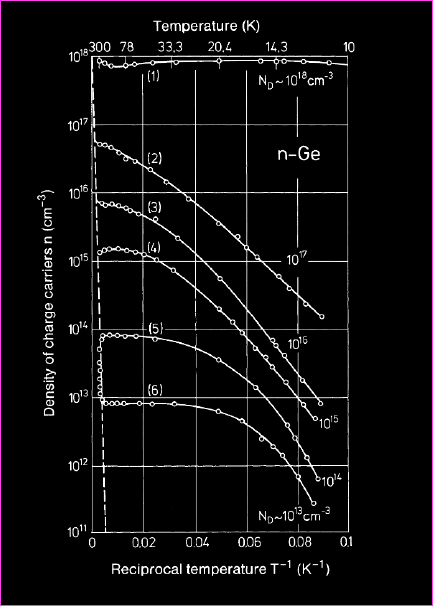
\includegraphics[scale=0.5]{images/Ge dopado.png}
\end{figure}
\end{center}
A primeira coisa que eu notei ao observar a imagem, é que no caso do nosso semicondutor puro, intrínseco, a densidade de portadores delétrons só começa a ser relevante a partir de altas temperatura. Supondo que a função que descreve a densidade dos portadores de elétrons seja contínua, e a "tendência" da função seja a mesma, é possível perceber que a densidade dos portadores de elétrons do semicondutor intrínseco para baixas temperaturas fica praticamente perto de zero, sendo negligenciável se comparado com sua versão dopada. Dessa forma, o nosso semicondutor à baixas temperaturas age basicamente como um isolante. Ao introduzirmos uma dopagem tipo-n no nosso Ge, temos mais elétrons disponíveis. Analisando o impacto da diferentes concentrações de dopantes e temperatura na densidade dos portadores de cargas, é possível notar-se algumas coisas. Primeiro, a é que parecem haver três "regimes" que determinam a densidade dos portadores de carga. Em baixas temperaturas, temos que $n << N_d$, e para baixas concentrações de $N_D$, o crescimento de $n$ com a temperatura parece ocorrer de maneira logarítima, até que chegamos à situação onde $n = N_D$. Nessa situação a variação de temperatura não afeta muito $n$, até que chegamos no regime de altas temperaturas e $n>N_D$. Nesse caso, podemos presumir que a temperatura foi o suficiente para ionizar os átomos, fazendo com que mais elétrons vão para a banda de condução, deixando buracos na banda de valência. É interessante notar que o aumento de concentração de dopantes faz com que o comportamento da função no gráfico $n \times K$ seja cada vez mais linear. Porém, quando chegamos em uma concentração tão alta de dopante, $N_D = 10^{18}$, praticamente a densidade de portadores de cargas é uma constante. Eu pressuponho que isso ocorre pelo fato da quantitade de elementos dopantes serem extremamente maiores do que a quantidade de átomos de Germânio.
  
\item Um semicondutor com um bandgap Eg = 1 eV e com as massas efetivas dos elétrons e dos buracos iguais à massa do elétrons livre, $m^∗_e = m^∗_h = m_0$, é dopado tipo-p com concentração de elementos aceitadores $p = 10^{18} cm^{−3}$.O nível de energia dos aceitadores é localizado em 0.2 eV acima da banda de valência do material.

  \begin{enumerate}
    \item mostre que a condução intrínseca (não dopado) deste material é desprezível à temperatura de 300 K

      Para mostrar que a conduão intrínseca deste material é desprezível à temperatura de 300K, podemos nos lembrar do fato passsado na nota de aula que todo elétron na banda de condução está relacionado a um buraco na banda de valência:

      \begin{equation}
          n = p = 24\left(\frac{k_BT}{2\pi\hbar^2}\right)^{3/2}(m_e^*m_h^*)^{3/4}e^{-E_g/2k_BT} 
      \end{equation}
      
      Substituindo os valores, parte a parte, obtemos o seguinte:

      \begin{center}
        \begin{align*}
          & k_B  \approx 8,617 \times 10^{-5}eV/K\\
          & k_BT  \approx 0,02585eV\\
          & \frac{E_g}{2k_BT}  \approx \frac{1 eV}{2 \times 0,02585 eV} \approx 19,34\\
          & e^{-\frac{E_g}{2k_BT}}  \approx e^{-19,34} \approx 3,9 \times 10^{-9}
        \end{align*}
      \end{center}
        Agora precisamos analisar o fator anterior à essa exponencial. Lembrando que $m^*_e = m^*_h = m_0$ (e p
        ulando algumas etapas do cálculo...), temos que:

        $$24\left(\frac{k_BT}{2\pi\hbar^2}\right)^{3/2}(m_e^*m_h^*)^{3/4}e^{-E_g/2k_BT} \approx (2 \ a \ 5) \times 10^{19}cm^{-3}$$

        Sendo assim, obtemos:

        $$n \approx (2 \ a \ 5)\times 10^{19} \times 3,9 \times 10^{-9} \approx (0,8 \ a \ 2) \times 10^{11}cm^{-3}$$
         
        Como a concentração de portadores de carga é 7 ordens de magnitudde menor do que a densidade de portadores no material dopado, podemos dizer que é sua condução intrínseca é desprezível.
        
      \item calcule a condutividade (\sigma) deste material à temperatura ambiente ($300 K$), dada uma mobilidade dos buracos de $\mu_p = 100 cm^2/Vs$ à $300 K$

        Sabendo que $\sigma = qp\mu_p$, podemos substituir os valores:

        $$\sigma = \left(1,6\times 10^{-19}A\cdot s\right) \times \left(10^{18}cm^{-3}\right) \left(100cm^2/V\cdot s\right) \approx 16 S/cm$$

        \item Faça um gráfico do logaritmo da concentração de buracos, ln(p), em função da temperatura recíproca (1/T) para intervalos de temperatura entre 100 K e 1000 K.

\begin{figure}[htbp]
  \centering
  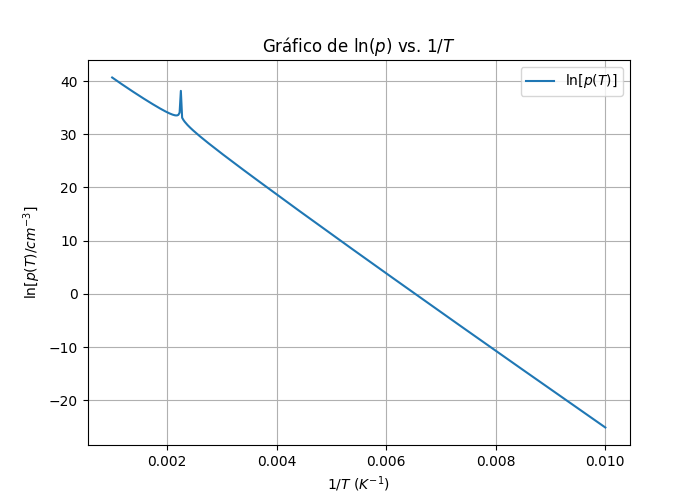
\includegraphics[scale=0.5]{images/gráfico.png}
\end{figure}

  \end{enumerate}

 \item Calcule a distância energética entre o nível de Fermi ($E_F$) e o meio do gap de energia para o silício puro e para o GaAs em 300 K. Explique o porque $E_F$ não é no meio do gap de energia. 

Como vimos nas notas de aula, temos que:\\
\\
\begin{equation}
  n = 2\left(\frac{2m_e^*k_BT}{2\pi\hbar^2}\right)^{3/2}e^{(\mu - E_c)/k_BT}
\end{equation}

Vamos definir que:

$$N_C = 2\left(\frac{2m_e^*k_BT}{2\pi\hbar^2}\right)^{3/2}$$

De maneira análoga, também definimos o $N_V$. Então podemos mostrar que $n$ é:
\begin{equation}
  n = N_Ce^{(\mu - E_C)/(k_BT)}, \ \ p = N_Ve^{(E_V - \mu)/k_BT} 
\end{equation}

Como $n = p = n_i$, podemos dizer que $n_i = \sqrt{np}$, ou seja:

$$n_i = \sqrt{N_CN_V}e^{-E_g/2k_BT}$$

Porém, sabemos que no semicondutor intrínseco $n = p = n_i$, dessa forma, podemos também dizer que:

$$n_i = N_C e^{\frac{\mu - E_C}{k_BT}}$$

Igualando as duas expressões para $n_i$, obtemos:

$$e^{(\mu - E_C)/k_BT} = \left(\frac{N_V}{N_C}\right)^{1/2}e^{-E_g/(2k_BT)}\\
\\
\Implies \frac{\mu - E_C}{k_BT} = \frac{1}{2}\ln{\left(\frac{N_V}{N_C}\right)} - \frac{E_g}{2k_BT}\\
\\
\Implies \mu = E_C - \frac{E_g}{2} + \frac{k_BT}{2}\ln{\left(\frac{N_V}{N_C}\right)}$$

Mas nós sabemos que $\mu = E_{Fi}$ (nível de fermi intrínseco), e que $E_g = E_C - E_V$, logo, obtemos que:

\begin{equation}
  E_{Fi} = \frac{E_C + E_V}{2} + \frac{k_BT}{2}\ln{\left(\frac{N_V}{N_C}\right)} 
\end{equation}

Resolvendo a questão, para o Silício, temos que o gap a 300K: $E_g \approx 1.12eV,\  m_e^*\approx 1.10m_0, \ m_h^* \approx 0.56$. Desse modo a razão $m_h^*/m_e^* \approx 0.55$. Ao substituir os valores, temos então que a energia de fermi estará um pouco acima da enenergia de gap.

Fazendo o mesmo para o GaAs, obtemos que a razão entre as massas efetivas $\approx 5$, ou seja, a energia de fermi está bem distante do gap.
\end{enumerate}
